
%(BEGIN_QUESTION)
% Copyright 2010, Tony R. Kuphaldt, released under the Creative Commons Attribution License (v 1.0)
% This means you may do almost anything with this work of mine, so long as you give me proper credit

Determine the temperature of the RTD, given a measured voltage of $-59.7$ millivolts between test points {\bf C} and {\bf D} in this circuit:

$$\includegraphics[width=15.5cm]{i00166x01.eps}$$

Assume a 100 $\Omega$ RTD with $\alpha = 0.00392$.

\underbar{file i00166}
%(END_QUESTION)





%(BEGIN_ANSWER)

$R_{RTD}$ = 107.256 $\Omega$

\vskip 10pt

$T$ = 65 degrees Fahrenheit (from table)

\vskip 10pt

$T$ = 65.32 degrees Fahrenheit (from formula)

%(END_ANSWER)





%(BEGIN_NOTES)


%INDEX% Measurement, temperature: RTD (2-wire with cable resistance)

%(END_NOTES)

